\section{Schnorr身份识别协议}

我们首先描述一种称为\textbf{Schnorr身份识别}的安全的身份识别协议。如果假定离散对数问题是困难的,那么该协议对窃听攻击是安全的。

令 $\mathbb{G}$ 是一个 $q$ 阶循环群,其中 $q$ 是素数,$g\in\mathbb{G}$ 是一个生成元。假设证明者 $P$ 有一个私钥 $\alpha\in\mathbb{Z}_q$,且与之对应的公钥为 $u=g^{\alpha}\in\mathbb{G}$。为了向验证者 $V$ 证明自己的身份,$P$ 想让 $V$ 相信自己知道 $\alpha$。最简单的方法是 $P$ 直接将 $\alpha$ 发送给 $V$。这个方法其实就是我们在\ref{sec:18-3} 中讨论过的口令协议版本 1,此时函数 $H(\alpha):=g^\alpha$扮演单向函数的角色。尽管这个协议提供了针对直接攻击的安全性,但它对窃听攻击是完全不安全的。相对, Schnorr 协议是一个经过巧妙设计的交互式协议,它允许 $P$ 说服 $V$ 相信自己知道以 $g$ 为基数的离散对数 $u$,但又并不需要真的将这个值发送给 $V$。

下面是它的工作原理。令 $\mathcal{C}\subset\mathbb{Z}_q$,则Schnorr身份识别协议 $\mathcal{I}_{\rm sch}=(G,P,V)$ 的原理如下:
\begin{itemize}
	\item 密钥生成算法 $G$ 按如下方式运行:
		\[
		\alpha\overset{\rm R}\leftarrow\mathbb{Z}_q,
		\quad
		u\leftarrow g^\alpha
		\]
		验证密钥为 $vk:=u$,私钥为 $sk:=\alpha$。
	\item $P$ 与 $V$ 之间的协议按照下面的方式运行。其中证明者 $P$ 由 $sk=\alpha$ 初始化,验证者 $V$ 由 $vk=u$ 初始化:
	\begin{enumerate}
		\item $P$ 计算 $\alpha_{\rm t}\overset{\rm R}\leftarrow\mathbb{Z}_q$,$u_{\rm t}\leftarrow g^{\alpha_{\rm t}}$,并将 $u_{\rm t}$ 发送给 $V$;
		\item $V$ 计算 $c\overset{\rm R}\leftarrow\mathcal{C}$,并将 $c$ 发送给 $P$;
		\item $P$ 计算 $\alpha_{\rm z}\leftarrow \alpha_{\rm t}+\alpha c\in \mathbb{Z}_q$,并将 $\alpha_{\rm z}$ 发送给 $V$;
		\item $V$ 检查 $g^{\alpha_{\rm z}}=u_{\rm t}\cdot u^c$ 是否成立,如果成立就输出 $\mathsf{accept}$,否则输出 $\mathsf{reject}$。
	\end{enumerate}
\end{itemize}
图 \ref{fig:19-1} 展示了该协议的工作流程。

\begin{figure}
  \centering
%  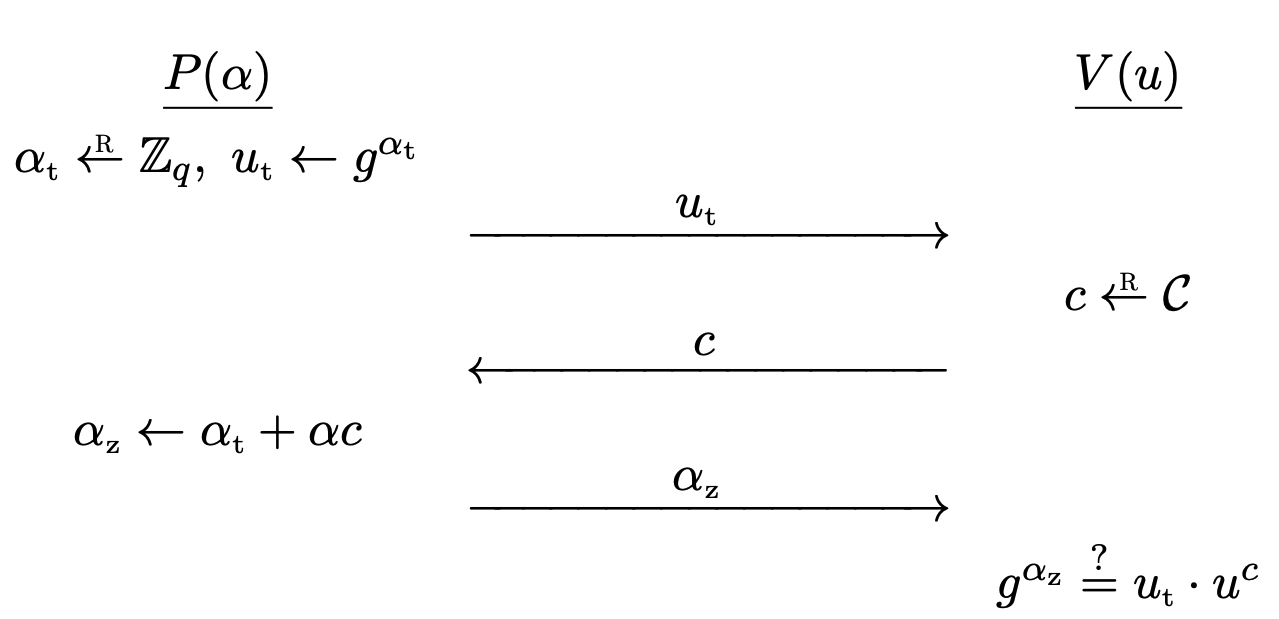
\includegraphics[width=0.55\linewidth]{figures/chapter19/fig1.png}
  

\tikzset{every picture/.style={line width=0.75pt}} %set default line width to 0.75pt        

\begin{tikzpicture}[x=0.75pt,y=0.75pt,yscale=-1,xscale=1]
%uncomment if require: \path (0,181); %set diagram left start at 0, and has height of 181

%Straight Lines [id:da4291410001374951] 
\draw  [->] (145,50) -- (305,50) ;
%Straight Lines [id:da21267819385876896] 
\draw  [<-] (145,90) -- (305,90) ;
%Straight Lines [id:da2885379053085584] 
\draw  [->] (145,130) -- (305,130) ;
%Straight Lines [id:da7969870205376979] 
\draw [line width=0.5]    (55,18) -- (85,18) ;
%Straight Lines [id:da6374733568626931] 
\draw [line width=0.5]    (335,18) -- (365,18) ;

% Text Node
\draw (70,10) node    {$P( \alpha )$};
% Text Node
\draw (70,30) node    {$\alpha _{\mathrm{t}}\overset{\mathrm{R}}{\leftarrow }\mathbb{Z}_{q} ,\ u_{\mathrm{t}}\leftarrow g^{\alpha _{\mathrm{t}}}$};
% Text Node
\draw (350,70) node    {$c\overset{\mathrm{R}}{\leftarrow }\mathcal{C}$};
% Text Node
\draw (70,110) node    {$\alpha _{\mathrm{z}}\leftarrow \alpha _{\mathrm{t}} +\alpha c$};
% Text Node
\draw (350,150) node    {$g^{\alpha _{\mathrm{z}}}\overset{?}{=} u_{\mathrm{t}} \cdot u^{c}$};
% Text Node
\draw (350,10) node    {$V( u)$};
% Text Node
\draw (225,46.6) node [anchor=south] [inner sep=0.75pt]    {$u\mathrm{_{t}}$};
% Text Node
\draw (225,86.6) node [anchor=south] [inner sep=0.75pt]    {$c$};
% Text Node
\draw (225,126.6) node [anchor=south] [inner sep=0.75pt]    {$\alpha _{\mathrm{z}}$};


\end{tikzpicture}
  \caption{Schnorr身份识别协议}
  \label{fig:19-1}
\end{figure}

$P(\alpha)$ 和 $V(u)$ 之间的一次交互产生一个\textbf{对话 (conversation)} $(u_{\rm t},c,\alpha_{\rm z})\in \mathbb{G}\times \mathcal{C}\times \mathbb{Z}_q$。如果 $V$ 的检查通过,即$g^{\alpha_{\rm z}}=u_{\rm t}\cdot u^c$ 成立,我们就称该对话为 \textbf{$u$ 的接受对话 (accepting conversation for $u$)}。不难看出,$P$ 和 $V$ 之间的交互总是能够产生一个接受对话,因为如果有 $u_{\rm t}=g^{\alpha_{\rm t}}$ 且 $\alpha_{\rm z}=\alpha_{\rm t}+\alpha c$,则有:
\[
g^{\alpha_{\rm z}}=g^{\alpha_{\rm t}+\alpha c}=g^{\alpha_{\rm t}}\cdot (g^\alpha)^c=u_{\rm t}\cdot u^c
\]
因此,Schnorr 协议能够满足身份识别协议所必需的基本正确性要求。

我们称集合 $\mathcal{C}$ 为\textbf{挑战空间 (challenge space)}。为了满足安全需求,我们要求 $|\mathcal{C}|$ 是超多项式的。事实上我们可以简单地取 $\mathcal{C}$ 为 $\mathbb{Z}_q$,但是技术上也可以允许更小的挑战空间。尽管我们最终会证明Schnorr协议在DL假设下对窃听攻击是安全的,但我们现在先从一个更简单的定理开始,它只证明了Schnorr协议对\emph{直接}攻击的安全性(攻击游戏 \ref{game:18-1})。

在证明这一点时,我们将表明,任何能够以不可忽略的概率成功执行直接仿冒攻击的对手,都能被转换成一个从验证密钥 $u$ 中高效地恢复私钥 $\alpha$的算法。由于这个原因,Schnorr的协议有时也被称为离散对数的知识证明。

\begin{theorem}\label{theo:19-1}
	基于 $\mathbb{G}$ 上的离散对数假设,假设 $N:=|\mathcal{C}|$ 是超多项式的,Schnorr 身份认证协议对直接攻击是安全的。
	\begin{quote}
		特别地,假设 $\mathcal{A}$ 是一个有效冒充对手,它通过攻击游戏 \ref{game:18-1} 中的直接攻击方式攻击 $\mathcal{I}_{\rm sch}$ 的优势为 $\epsilon:={\rm ID1\mathsf{adv}}[\mathcal{A},\mathcal{I}_{\rm sch}]$。那么必然存在一个有效的离散对数对手 $\mathcal{B}$,其运行时间大致是 $\mathcal{A}$ 的两倍,其优势为 $\epsilon':={\rm DL\mathsf{adv}}[\mathcal{B},\mathbb{G}]$,并且有:
	\end{quote}
	\begin{equation}\label{eq:19-1}
		\epsilon'\geq \epsilon^2-\frac{\epsilon}{N}
	\end{equation}
	\begin{quote}
		也即:
	\end{quote}
	\begin{equation}\label{eq:19-2}
		\epsilon\leq\frac{1}{N}+\sqrt{\epsilon'}
	\end{equation}
\end{theorem}

\begin{proof}[证明思路]
假设攻击游戏 \ref{game:18-1} 中的对手 $\mathcal{A}$ 在攻击 $\mathcal{I}_{\rm sch}$ 时有优势 $\epsilon$。在该游戏中,挑战者生成验证密钥 $u=g^\alpha$。在对手 $\mathcal{A}$ 的冒充尝试中,它基于某个任意的对手策略生成了协议的第一条交互信息 $u_{\rm t}$。为了赢得游戏,对手 $\mathcal{A}$ 必须用一个有效应答 $\alpha_{\rm z}$ 来响应随机挑战 $c\in\mathcal{C}$,使得 $g^{\alpha_{\rm z}}=u_{\rm t}\cdot u^c$。直观地讲,如果 $\mathcal{A}$ 能以概率 $\epsilon$ 对一个这样的随机挑战产生一个有效应答,那么它就应该能以概率 $\epsilon^2$ 对\emph{两个}随机挑战产生一个有效的应答。要使这一直觉变得严谨,需要一个有点技术性的论证,我们将在随后的引理中给出。

下面,我们先介绍如何使用 $\mathcal{A}$ 计算随机数 $u\in\mathbb{G}$ 的离散对数。我们使用 $u$ 作为 $\mathcal{I}_{\rm sch}$ 的验证密钥,并让 $\mathcal{A}$ 生成协议的第一条交互 $u_{\rm t}$。然后我们向 $\mathcal{A}$ 提供一个随机挑战 $c$,并希望 $\mathcal{A}$ 产生一个有效应答 $\alpha_{\rm z}$。如果这确实发生了,我们就将 $\mathcal{A}$ 的内部状态``回溯"到它刚刚生成 $u_{\rm t}$ 后的那一刻,然后给 $\mathcal{A}$ 提供另一个随机挑战 $c'$,并希望 $\mathcal{A}$ 产生另一个有效应答 $\alpha_{\rm z}'$。

如果上面这些都发生了,那么对于一个给定的验证密钥 $u$,我们就得到了两个接受对话 $(u_{\rm t},c,\alpha_{\rm z})$ 和 $(u_{\rm t},c',\alpha_{\rm z}')$,且这两个对话的第一条交互 $u_{\rm t}$ 相同。此外,由于 $\mathcal{C}$ 是超多项式的,因此我们可以以压倒性的概率得到 $c'\neq c$ 。基于以上信息,我们可以很容易地计算出 ${\rm \mathsf{Dlog}}_gu$。事实上,由于上面的两个对话都是接受对话,我们有下面两个等式:
\[
g^{\alpha_{\rm z}}=u_{\rm t}\cdot u^c,
\quad
g^{\alpha_{\rm z}'} =u_{\rm t}\cdot u^{c'}
\]
用第一式除以第二式, $u_{\rm t}$ 就被抵消了,于是我们有:
\begin{equation}\label{eq:19-3}
	g^{\Delta\alpha}=u^{\Delta c}
\end{equation}
其中$\Delta\alpha:=\alpha_{\rm z}-\alpha_{\rm z}'$,$\Delta c:=c-c'$。由于 $\Delta c\neq 0$,且循环群 $\mathbb{G}$ 的阶 $q$ 是素数,所以倒数 ${1}/{\Delta c}$ 存在于 $\mathbb{Z}_q$ 中。我们可以将式 \ref{eq:19-3} 中等式的左右两边都升阶 ${1}/{\Delta c}$,于是有:
\[
g^{{\Delta\alpha}/{\Delta c}}=u
\]
因此,我们可以有效计算离散对数 ${\rm \mathsf{Dlog}}_gu$,其值为 ${\Delta\alpha}/{\Delta c}$。

读者应该注意到,这里提出的从两个接受对话中提取离散对数的技术,与事实 10.3 中使用的想法基本相同。事实上,使用 10.6.1 节中的术语,我们可以看到 $(\alpha_{\rm z},-c)$ 和 $(\alpha_{\rm z}',-c')$ 是 $u_{\rm t}$ 相对于$g$ 和 $u$ 的不同表示。事实 10.3 告诉了我们如何从这两个表示中计算出 ${\rm \mathsf{Dlog}}_gu$。
\end{proof}

这个定理与我们在本文中迄今为止所介绍的所有其他安全定理有着质的不同。事实上,在这个定理的证明中,虽然我们表明每个攻击 $\mathcal{I}_{\rm sch}$ 的对手 $\mathcal{A}$ 都可以转化为破解离散对数问题的对手 $\mathcal{B}$,但我们构造的对手 $\mathcal{B}$ \emph{并不是} $\mathcal{A}$ 的基本包装器,因为对手 $\mathcal{B}$ 要运行 $\mathcal{A}$ \emph{两次}。此外,这个定理在量上也是不同的,因为安全归约根本就不是很严密:如果 $\mathcal{A}$ 以概率 $\epsilon$ 获胜,那么 $\mathcal{B}$ 只能保证以 $\approx\epsilon^2$ 的概率获胜。

因此,为了使上述想法更严谨,我们需要先引入下面的引理:

\begin{lemma}[回溯引理]\label{theo:19-2}
令 $S$ 和 $T$ 是两个非空有限集,$f:S\times T\to\{0,1\}$ 是一个函数。令 $\mathsf{X}$、$\mathsf{Y}$ 和 $\mathsf{Y}'$ 是相互独立的随机变量,其中 $\mathsf{X}$ 在集合 $S$ 中取值,$\mathsf{Y}$ 和 $\mathsf{Y}'$ 都在 $T$ 上均匀分布。令 $\epsilon:=\Pr[f(\mathsf{X},\mathsf{Y})=1]$,$N:=|T|$,则有:
\[
\Pr[f(\mathsf{X},\mathsf{Y})=1\land f(\mathsf{X},\mathsf{Y}')=1\land \mathsf{Y}\neq\mathsf{Y}']\geq\epsilon^2-\frac{\epsilon}{N}
\]
\end{lemma}

\begin{proof}
	对于每个 $s\in S$,令 $g(s):=\Pr[f(s,\mathsf{Y})=1]$。首先,我们可以观察到 $E[g(\mathsf{X})]=\epsilon$,这是因为:
	\begin{equation*}
		\begin{aligned}
			E[g(\mathsf{X})]
			&=\sum_{s\in S}g(s)\Pr[\mathsf{X}=s]=\sum_{s\in S}\Pr[f(s,\mathsf{Y})=1]\Pr[\mathsf{X}=s]\\
			&=\sum_{s\in S}\Pr[f(s,\mathsf{Y})=1\land \mathsf{X}=s] \text{ \emph{(独立性)}}\\
			&=\sum_{s\in S}\Pr[f(\mathsf{X},\mathsf{Y})=1\land \mathsf{X}=s]\\
			&=\Pr[f(\mathsf{X},\mathsf{Y})=1] \text{ \emph{(全概率)}}\\
			&=\epsilon
		\end{aligned}
	\end{equation*}
	
	其次,考虑一个固定的 $s∈S$,令 $\mathcal{U}_s$ 为 $f(s,\mathsf{Y})=1\land f(s,\mathsf{Y}')=1\land \mathsf{Y}\neq\mathsf{Y}'$ 成立的事件,我们称:
	\[
	\Pr[\mathcal{U}_s]=g(s)^2-\frac{g(s)}{N}
	\]
	为了证明这一点,令 $N_s$ 是满足 $f(s, t)=1$ 的 $t\in T$ 的数量,那么有 $N_s$ 种方法可以选择满足 $f(s,\mathsf{Y})=1$ 的 $\mathsf{Y}$。而对于每个 $\mathsf{Y}$ 的选择,有 $N_s-1$ 种方法可以选择满足 $f(s,\mathsf{Y}')=1\land \mathsf{Y}\neq\mathsf{Y}'$ 的 $\mathsf{Y}'$。由于 $g(s)={N_s}/{N}$,因此我们有:
	\[
	\Pr[\mathcal{U}_s]=\frac{N_s(N_s-1)}{N^2}=\frac{N_s^2}{N^2}-\frac{N_s}{N^2}=g(s)^2-\frac{g(s)}{N}
	\]

	最后,令 $\mathcal{U}$ 为 $f(\mathsf{X},\mathsf{Y})=1\land f(\mathsf{X},\mathsf{Y}')=1\land \mathsf{Y}\neq\mathsf{Y}'$ 成立的事件,我们有:
	\begin{equation*}
		\begin{aligned}
			\Pr[\mathcal{U}]
			&=\sum_{s\in S}\Pr[\mathcal{U}\land\mathsf{X}=s]\text{ \emph{(全概率)}}\\
			&=\sum_{s\in S}\Pr[f(s,\mathsf{Y})=1\land f(s,\mathsf{Y}')=1\land \mathsf{Y}\neq\mathsf{Y}'\land\mathsf{X}=s]\\
			&=\sum_{s\in S}\Pr[f(s,\mathsf{Y})=1\land f(s,\mathsf{Y}')=1\land \mathsf{Y}\neq\mathsf{Y}']\cdot\Pr[\mathsf{X}=s]\text{ \emph{(独立性)}}\\
			&=\sum_{s\in S}\Pr[\mathcal{U}_s]\cdot\Pr[\mathsf{X}=s]=\sum_{s\in S}[g(s)^2-\frac{g(s)}{N}]\cdot\Pr[\mathsf{X}=s]\\
			&=E[g(\mathsf{X})^2]-\frac{g(\mathsf{X})}{N}\\
			&\geq E[g(\mathsf{X})]^2-\frac{E[g(s)]}{N}=\epsilon^2-\frac{\epsilon}{N}
		\end{aligned}
	\end{equation*}
	上面我们使用了这样一个一般事实:对于任意随机变量 $\mathsf{Z}$ 都有 $E[\mathsf{Z}^2]\geq E[\mathsf{Z}]^2$,在这里我们的这个 $\mathsf{Z}=g(\mathsf{X})$。这是詹森不等式的一个特例。
\end{proof}

\begin{proof}[定理 \ref{theo:19-1} 的证明]
	利用具有优势 $\epsilon$ 的冒充对手 $\mathcal{A}$ ,我们能够建立一个具有优势 $\epsilon'$ 的 DL 对手 $\mathcal{B}$,如下所示。对手 $\mathcal{B}$ 从其挑战者那里得到一个 DL 问题实例 $u = g^\alpha$,而我们的目标是让 $\mathcal{B}$ 在 $\mathcal{A}$ 的帮助下计算出 $\alpha$。$\mathcal{B}$ 的计算过程可以分为两个阶段。

在第一阶段,$\mathcal{B}$ 扮演 $\mathcal{A}$ 的挑战者的角色,将 $u$ 的值交给 $\mathcal{A}$ 作为验证公钥。在这一步中,$\mathcal{B}$ 的目标是计算出两个具有不同挑战的 $u$ 的接受对话,即:
\[
(u_{\rm t},c,\alpha_{\rm z}),
\quad
(u_{\rm t},c',\alpha_{\rm z}')
\]
其中:
\[
g^{\alpha_{\rm z}}=u_{\rm t}\cdot u^c,
\quad
g^{\alpha_{\rm z}'}=u_{\rm t}\cdot u^{c'},
\quad
c\neq c'
\]

以下是 $\mathcal{B}$ 做到这一点的方法:
\begin{enumerate}
	\item $\mathcal{A}$ 扮演证明者,并将 $u_{\rm t}$ 发送给扮演验证者的 $\mathcal{B}$;
	\item $\mathcal{B}$ 向 $\mathcal{A}$ 发送一个随机数 $c\in\mathcal{C}$;
	\item $\mathcal{A}$ 向 $\mathcal{B}$ 发送 $\alpha_{\rm z}$;
	\item $\mathcal{B}$ 对 $\mathcal{A}$ 进行``回溯"操作,使 $\mathcal{A}$ 的内部状态与步骤 1 结束时完全相同,然后 $\mathcal{B}$ 向 $\mathcal{A}$ 发送一个新的随机数 $c'\in\mathcal{C}$;
	\item $\mathcal{A}$ 向 $\mathcal{B}$ 发送 $\alpha_{\rm z}'$。
\end{enumerate}
下面我们应用回溯引理 \ref{theo:19-2}。在该引理中,随机变量 $\mathsf{Y}$ 与挑战 $c$ 对应,$\mathsf{Y}'$ 与挑战 $c'$ 对应,$\mathsf{X}$ 与 $\mathcal{A}$ 、$\mathcal{B}$ 和 $\mathcal{B}$ 的挑战者的所有其他随机选择对应,具体包括群 $\mathbb{G}$ 和群元素 $g,u,u_t\in\mathbb{G}$。当产生的对话是 $u$ 的一个接受对话时,引理中的函数 $f$ 为 $1$,否则就为 $0$。因此,如果 $(u_{\rm t},c,\alpha_{\rm z})$ 是 $u$ 的接受对话,则 $f(\mathsf{X},\mathsf{Y})=1$,如果 $(u_{\rm t},c',\alpha_{\rm z}')$ 是 $u$ 的接受性对话,则 $f(\mathsf{X},\mathsf{Y}')=1$。应用该引理,我们发现 $\mathcal{B}$ 得到两个不同挑战的接受对话的概率至少为 $\epsilon^2-{\epsilon}/{N}$。

所以现在假设 $\mathcal{B}$ 已经成功计算出两个这样的接受对话 $(u_{\rm t},c,\alpha_{\rm z})$ 和 $(u_{\rm t},c',\alpha_{\rm z}')$。在第二阶段,$\mathcal{B}$ 用这两个对话来计算 $\alpha$。事实上,正如在上面的证明思路中已经讨论过的,我们可以计算$\alpha={\Delta\alpha}/{\Delta c}$,其中$\Delta\alpha:=\alpha_z-\alpha_z'$,$\Delta c:=c-c'$。

这就得到了式 \ref{eq:19-1}。下面我们论证式 \ref{eq:19-2} 可由式 \ref{eq:19-1} 推出。为此,我们不妨假设 $\epsilon\geq{1}/{N}$,否则式 \ref{eq:19-2} 显然是成立的。因此我们有:
\[
\begin{aligned}
	(\epsilon-\frac{1}{N})^2
	&=\epsilon^2-\frac{2\epsilon}{N}+\frac{1}{N^2}\leq\epsilon^2-\frac{2\epsilon}{N}+\frac{\epsilon}{N} \text{\emph{ (因为 }}\epsilon\geq\frac{1}{N}\text{\,)}\\
	&=\epsilon^2-\frac{\epsilon}{N}\leq \epsilon' \text{ \emph{(式} \ref{eq:19-1}\,\emph{)}}
\end{aligned}
\]
因此式 \ref{eq:19-2} 得证。

回顾一下,我们展示了如何从恶意验证者 $\mathcal{A}$ 中有效地\emph{提取}私钥 $\alpha$,进而证明了针对直接攻击的安全性。这使我们能够利用恶意验证者来解决$\mathbb{G}$中的离散对数问题。我们的\emph{提取器}通过回溯证明者的状态来获得两个接受对话 $(u_{\rm t},c,\alpha_{\rm z})$ 和 $(u_{\rm t},c',\alpha_{\rm z}')$,其中 $c\neq c'$。在安全性证明中回溯证明者 $\mathcal{A}$ 是可能的,因为我们完全控制了 $\mathcal{A}$ 的执行环境。在现实世界中,由于不能对诚实证明 $P$ 进行回溯,攻击者就不能使用这种策略从 $P$ 那里提取私钥。
\end{proof}

\subsection{诚实验证者零知识和针对窃听的安全性}\label{subsec:19-1-1}

我们已经证明了在离散对数假设下,Schnorr 协议对\emph{直接}攻击是安全的。事实上在相同的假设下,Schnorr 协议对于\emph{窃听}攻击也是安全的。现在,在某次窃听攻击中,对手获得了 $vk$ 和一张记录列表,该表的内容是$P$(在输入$sk$上)与 $V$(在输入$vk$上)之间的若干对话。我们的想法是证明这些对话对于对手来说没有任何帮助,因为在给定 $vk$ 而没有给定 $sk$ 的情况下,对手也可以自己有效地生成这些对话。如果我们能证明这一点,我们也就大功告成了。事实上,假设 $\mathcal{A}$ 是一个对手,它通过窃听成功发动仿冒攻击的优势是不可忽略不计的。然后,我们用另一个对手 $\mathcal{B}$ 来替代 $\mathcal{A}$,它的工作方式与 $\mathcal{A}$ 是一样的,只是现在 $\mathcal{B}$ 自己生成了对话列表,而不是从挑战者那里获取记录。这样,$\mathcal{B}$ 就发动了一个直接攻击,但是它与发动仿冒攻击的 $\mathcal{A}$ 具有相同的优势。

下面,我们将上面的想法扩展到更一般的情况,引入\textbf{诚实验证者零知识} 的概念。

\begin{definition}
	令 $\mathcal{I}=(G,P,V)$ 是一个身份识别协议。如果存在一个有效的概率性算法 $Sim$(称为\textbf{模拟器 simulator})使得对于 $G$ 的任意可能输出 $(vk,sk)$,$Sim$ 在输入 $vk$ 上的输出分布与 $P$ (在输入$sk$上)与 $V$(在输入$vk$上) 之间对话记录的分布相同,我们就称 $\mathcal{I}$ 是\textbf{诚实验证者零知识 (honest verifier zero knowledge, HVZK)} 的。
\end{definition}

下面,我们对其中的一些术语进行说明。所谓``零知识"的意思是,对手从 $P$ 那里什么也学不到,因为对手可以在不知道 $sk$ 的情况下自己使用算法 $Sim$ 模拟对话。而``诚实验证者"表达了这样一个事实,即这种模拟只对 $P$ 和\emph{诚实的}验证者 $V$ 之间的对话有效,而对于\emph{非诚实}的验证者,比如\emph{主动}攻击中可能出现的验证者,都是无效的。零知识的概念,包括诚实验证者零知识以及许多其他的变体,还会出现在身份识别协议之外的许多其他类型的协议中。

\begin{theorem}\label{theo:19-3}
	如果一个身份识别协议 $\mathcal{I}=(G,P,V)$ 对于直接攻击是安全的,且该协议是 HVZK 的,那么该协议对于窃听攻击也是安全的。
	\begin{quote}
		特别地,如果 $\mathcal{I}$ 是带有模拟器 ${Sim}$ 的 HVZK,那么对于每一个通过攻击游戏 18.2 中的窃听攻击来攻击 $\mathcal{I}$ 的冒充对手 $\mathcal{A}$,如果 $\mathcal{A}$ 最多能获得 $Q$ 次交互记录,必然存在一个通过攻击游戏 \ref{game:18-1} 中的直接攻击来攻击 $\mathcal{I}$ 的对手 $\mathcal{B}$,其中 $\mathcal{B}$ 是一个围绕 $\mathcal{A}$ 的基本包装器,并且 $\mathcal{B}$ 最多运行 $Q$ 次 ${Sim}$,满足:
		\[
		{\rm ID2\mathsf{adv}}[\mathcal{A},\mathcal{I}]={\rm ID1\mathsf{adv}}[\mathcal{B},\mathcal{I}]
		\]
	\end{quote}
\end{theorem}

\begin{proof}
	$\mathcal{B}$ 的工作方式与 $\mathcal{A}$ 相同,只是它不是从挑战者那里获得交互记录,而是用 ${Sim}$ 自己生成交互记录。对手 $\mathcal{B}$ 的工作方式如图 \ref{fig:19-2} 所示。
\end{proof}

\begin{figure}
  \centering
  

\tikzset{every picture/.style={line width=0.75pt}} %set default line width to 0.75pt        

\begin{tikzpicture}[x=0.75pt,y=0.75pt,yscale=-0.9,xscale=0.9]
%uncomment if require: \path (0,369); %set diagram left start at 0, and has height of 369

%Shape: Rectangle [id:dp26654228996316176] 
\draw  [fill={rgb, 255:red, 255; green, 255; blue, 255 }  ,fill opacity=1 ][line width=1.2] [general shadow={fill=black,shadow xshift=2.25pt,shadow yshift=-2.25pt}] (10,80) -- (110,80) -- (110,300) -- (10,300) -- cycle ;
%Shape: Rectangle [id:dp7569838380400329] 
\draw  [fill={rgb, 255:red, 255; green, 255; blue, 255 }  ,fill opacity=1 ][line width=1.2] [general shadow={fill=black,shadow xshift=2.25pt,shadow yshift=-2.25pt}] (510,80) -- (550,80) -- (550,300) -- (510,300) -- cycle ;
%Shape: Rectangle [id:dp8533457962352082] 
\draw  [dash pattern={on 5.63pt off 4.5pt}][line width=1.2]  (260,40) -- (590,40) -- (590,340) -- (260,340) -- cycle ;
%Shape: Rectangle [id:dp9157199572503583] 
\draw   (25,245) -- (95,245) -- (95,285) -- (25,285) -- cycle ;
%Straight Lines [id:da21399463334844526] 
\draw    (60,337) -- (60,285) ;
\draw [shift={(60,340)}, rotate = 270] [fill={rgb, 255:red, 0; green, 0; blue, 0 }  ][line width=0.08]  [draw opacity=0] (7.14,-3.43) -- (0,0) -- (7.14,3.43) -- cycle    ;
%Straight Lines [id:da925421640822562] 
\draw    (507,110) -- (110,110) ;
\draw [shift={(510,110)}, rotate = 180] [fill={rgb, 255:red, 0; green, 0; blue, 0 }  ][line width=0.08]  [draw opacity=0] (7.14,-3.43) -- (0,0) -- (7.14,3.43) -- cycle    ;
%Straight Lines [id:da6618660867514581] 
\draw    (510,270) -- (116,270) ;
\draw [shift={(113,270)}, rotate = 360] [fill={rgb, 255:red, 0; green, 0; blue, 0 }  ][line width=0.08]  [draw opacity=0] (7.14,-3.43) -- (0,0) -- (7.14,3.43) -- cycle    ;
\draw [shift={(510,270)}, rotate = 180] [fill={rgb, 255:red, 0; green, 0; blue, 0 }  ][line width=0.08]  [draw opacity=0] (7.14,-3.43) -- (0,0) -- (7.14,3.43) -- cycle    ;
%Straight Lines [id:da6795099348296265] 
\draw    (310,150) -- (507,150) ;
\draw [shift={(510,150)}, rotate = 180] [fill={rgb, 255:red, 0; green, 0; blue, 0 }  ][line width=0.08]  [draw opacity=0] (7.14,-3.43) -- (0,0) -- (7.14,3.43) -- cycle    ;
%Straight Lines [id:da5247033753927413] 
\draw    (310,230) -- (507,230) ;
\draw [shift={(510,230)}, rotate = 180] [fill={rgb, 255:red, 0; green, 0; blue, 0 }  ][line width=0.08]  [draw opacity=0] (7.14,-3.43) -- (0,0) -- (7.14,3.43) -- cycle    ;

% Text Node
\draw (60,65) node   [align=left] {直接挑战者};
% Text Node
\draw (60,95) node    {$( sk,vk)\overset{\mathrm{R}}{\leftarrow } G$};
% Text Node
\draw (60,265) node    {$V( vk)$};
% Text Node
\draw (185,106.6) node [anchor=south] [inner sep=0.75pt]    {$vk$};
% Text Node
\draw (410,146.6) node [anchor=south] [inner sep=0.75pt]    {$Sim( vk)$};
% Text Node
\draw (410,226.6) node [anchor=south] [inner sep=0.75pt]    {$Sim( vk)$};
% Text Node
\draw (410,180) node    {$\vdots $};
% Text Node
\draw (385,267) node [anchor=south] [inner sep=0.75pt]   [align=left] {冒充尝试};
% Text Node
\draw (530,65) node   [align=left] {窃听对手 $\displaystyle \mathcal{A}$};
% Text Node
\draw (297,25) node   [align=left] {直接对手 $\displaystyle \mathcal{B}$};
% Text Node
\draw (62,340) node [anchor=west] [inner sep=0.75pt]   [align=left] {$\displaystyle \mathsf{accept}$ 或 $\displaystyle \mathsf{reject}$};


\end{tikzpicture}
  \caption{定理 \ref{theo:19-3} 的证明中的对手 $\mathcal{B}$}
  \label{fig:19-2}
\end{figure}

下面让我们回到 Schnorr 身份识别协议。

\begin{theorem}\label{theo:19-4}
	Schnorr 身份识别协议是 HVZK 的。
\end{theorem}

\begin{proof}
	证明的思路是在生成模拟对话 $(u_{\rm t},c,\alpha_{\rm z})$ 时,我们不需要像 $P$ 和 $V$ 之间的真实对话那样,按照给定的顺序生成对话中的消息。事实上,模拟器 ${Sim}$ 是以\emph{倒序}生成信息的。在输入 $vk=u$ 时,模拟器 ${Sim}$ 计算:
		\[
		\alpha_{\rm z}\overset{\rm R}\leftarrow\mathbb{Z}_q,
		\quad
		c\overset{\rm R}\leftarrow\mathcal{C},
		\quad
		u_{\rm t}\leftarrow\frac{g^{\alpha_{\rm z}}}{u^c}
		\]
	并输出对话 $(u_{\rm t},c,\alpha_{\rm z})$。
	
	现在我们论证 ${Sim}$ 在输入 $vk=u$ 上的输出具有正确的分布。一个关键性的观察是,在真实交互中,$c$ 和 $\alpha_{\rm z}$ 是相互独立的,$c$ 在 $\mathcal{C}$ 上均匀分布,而 $\alpha_z$ 在 $\mathbb{Z}_q$ 上均匀分布。此外,给定 $c$ 和 $\alpha_{\rm z}$,$u_{\rm t}$ 的值可由等式 $g^{\alpha_{\rm z}}=u_{\rm t}\cdot u^c$ 唯一确定。而这显然与模拟器的输出分布相同。
\end{proof}

作为一个推论,我们立即可以得到:

\begin{theorem}\label{theo:19-5}
	如果 Schnorr 身份识别协议对直接攻击是安全的,那么它对窃听攻击也是安全的。
	
	\begin{quote}
		特别地,对于每个通过攻击游戏 18.2 中的窃听攻击来攻击 $\mathcal{I}_{\rm sch}$ 的冒充对手 $\mathcal{A}$,都有一个通过攻击游戏 \ref{game:18-1} 中的直接攻击来攻击 $\mathcal{I}_{\rm sch}$ 的对手 $\mathcal{B}$,其中 $\mathcal{B}$ 是一个围绕 $\mathcal{A}$ 的基本包装器,满足:
		\[
		{\rm ID2\mathsf{adv}}[\mathcal{A},\mathcal{I}_{\rm sch}]=
		{\rm ID1\mathsf{adv}}[\mathcal{B},\mathcal{I}_{\rm sch}]
		\]
	\end{quote}
\end{theorem}

乍看之下,我们关于 Schnorr 协议的结论似乎是反直觉的,甚至可能是矛盾的。在只知道 $vk$ 的情况下,怎么可能既很难进行冒充攻击,又容易产生对话呢?答案是,在进行冒充攻击时,验证者 $V$ 主动地参与对话,而消息的时间和顺序至关重要:扮演证明者的对手必须在看到 $V$ 生成的挑战 $c$ \emph{之前}生成第一条消息 $u_{\rm t}$。然而,模拟器可以自由地以任何方便的顺序生成信息:在定理 \ref{theo:19-4} 的证明中,模拟器先生成了 $c$ 和 $\alpha_{\rm z}$,然后才计算 $u_{\rm t}$。这些结果表明,如果挑战空间很小,Schnorr 协议将是完全\emph{不安全}的:在冒充尝试中,对手可以使用模拟器准备一个接受对话 $(u_{\rm t},c,\alpha_{\rm z})$,然后将 $u_{\rm t}$ 发送给 $V$,然后希望 $V$ 选择的挑战等于其准备的挑战 $c$。如果真的是这样,对手就可以用 $\alpha_{\rm z}$ 应答从而使 $V$ 接受对话。因此,以 ${1}/{|\mathcal{C}|}$ 的优势破解 Schnorr 识别协议是很容易的。所以为了确保安全性,挑战空间的大小 $|\mathcal{C}|$ 必须是超多项式的。

Schnorr 识别协议对攻击游戏 18.3 中的\emph{主动}攻击是否安全是一个开放的问题:目前还没有已知的有效主动攻击,但也没有证据可以排除离散对数假设下的这种攻击。在本章的稍后部分,我们将介绍一个对Schnorr身份识别的细小变化,它被证明在DL假设下对主动攻击是安全的。